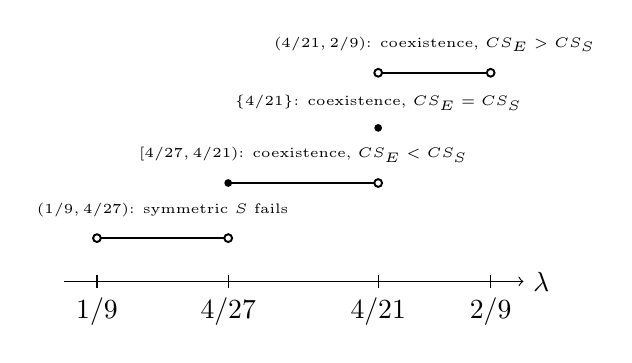
\begin{tikzpicture}[x=1.25cm,y=1cm]
\draw[->] (3.666667,0) -- (8.333333,0) node[right] {$\lambda$};
\draw (4.000000,0.08) -- (4.000000,-0.08) node[below] {$1/9$};
\draw (5.333333,0.08) -- (5.333333,-0.08) node[below] {$4/27$};
\draw (6.857143,0.08) -- (6.857143,-0.08) node[below] {$4/21$};
\draw (8.000000,0.08) -- (8.000000,-0.08) node[below] {$2/9$};
\draw[line width=0.7pt] (4.000000,0.55) -- (5.333333,0.55);
\draw[fill=white,line width=0.7pt] (4.000000,0.55) circle (1.4pt);
\draw[fill=white,line width=0.7pt] (5.333333,0.55) circle (1.4pt);
\node[align=center,font=\tiny] at (4.666667,0.91) {$(1/9,4/27)$: symmetric $S$ fails};
\draw[line width=0.7pt] (5.333333,1.25) -- (6.857143,1.25);
\fill (5.333333,1.25) circle (1.4pt);
\draw[fill=white,line width=0.7pt] (6.857143,1.25) circle (1.4pt);
\node[align=center,font=\tiny] at (6.095238,1.61) {$[4/27,4/21)$: coexistence, $CS_E<CS_S$};
\fill (6.857143,1.95) circle (1.4pt);
\node[align=center,font=\tiny] at (6.857143,2.27) {$\{4/21\}$: coexistence, $CS_E=CS_S$};
\draw[line width=0.7pt] (6.857143,2.65) -- (8.000000,2.65);
\draw[fill=white,line width=0.7pt] (6.857143,2.65) circle (1.4pt);
\draw[fill=white,line width=0.7pt] (8.000000,2.65) circle (1.4pt);
\node[align=center,font=\tiny] at (7.428571,3.01) {$(4/21,2/9)$: coexistence, $CS_E>CS_S$};
\end{tikzpicture}
